\documentclass[aspectratio=169]{beamer}

\mode<presentation>
{
  \usetheme{Madrid}
  \setbeamercovered{transparent}
}

\date{10 June 2024}

\frenchspacing

\usepackage[utf8]{inputenc}

\usepackage{fancyvrb}

\usepackage{times}
\usepackage[T1]{fontenc}

\title{BSRC REU GNU Radio tutorials}
\subtitle{Introduction}
\author{Daniel Estévez}

\institute
{}

\subject{}

\AtBeginSection[]
{
  \begin{frame}<beamer>{Outline}
    \tableofcontents[currentsection,currentsubsection]
  \end{frame}
}

\begin{document}

\frame{\titlepage}

\begin{frame}{GNU Radio}
  \begin{itemize}
    \item GNU Radio is an open source framework to do DSP for radio
      (communications, RADAR, radio astronomy...). Also useful for applications
      that do similar computing (even particle accelerators!).
    \item It comes with:
      \begin{itemize}
        \item A GUI application called ``GNU Radio companion'' where
             systems can be implemented by dragging and dropping blocks onto a
             canvas (making a ``flowgraph'')
        \item A rich library of processing blocks accessible both through GNU Radio
          companion, and C++ and Python APIs
        \item A ``runtime'', that moves data between these blocks and runs the
          code of each block
      \end{itemize}
    \item In the GNU Radio ecosystem there are out-of-tree modules, which
      implement new blocks that don't fit into or exist in the in-tree library
    \item There are also full applications that use GNU Radio for their DSP (for
      instance, GQRX, or QRadioLink)
  \end{itemize}
  
\includegraphics[width=0.4\textwidth]{gnuradio_logo}
\end{frame}

\begin{frame}{Making flowgraphs with GNU Radio companion}
  \begin{center}
    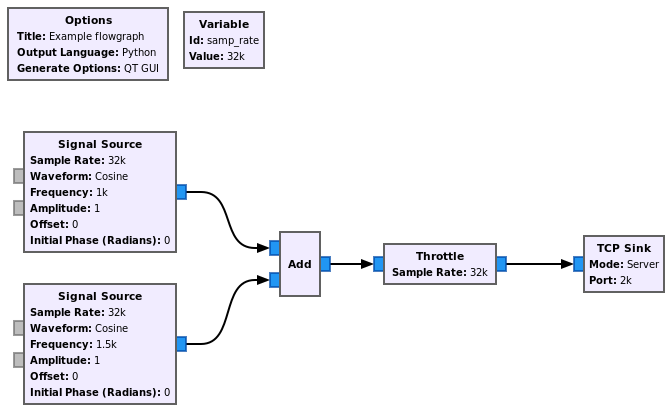
\includegraphics[width=0.8\textwidth]{example_flowgraph}
  \end{center}
\end{frame}

\begin{frame}{Making flowgraphs in Python}
  \begin{center}
    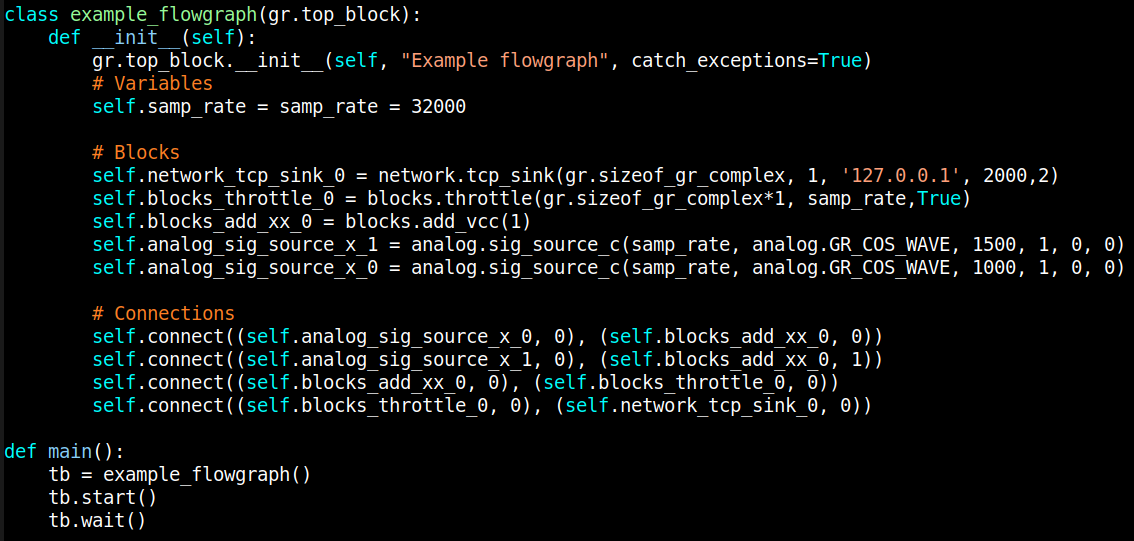
\includegraphics[width=\textwidth]{python_flowgraph}
  \end{center}
\end{frame}

\begin{frame}{Using GNU Radio in SETI and radio astronomy}
  Here are some applications in which GNU Radio is useful (or can be useful):
  \begin{itemize}
  \item Full backend for small radio telescopes
  \item RFI analysis and simulation
  \item Simulation of technosignatures and other signals of interest
  \item Prototyping signal processing algorithms
  \item Teaching signal processing
  \end{itemize}
\end{frame}

\end{document}


